%%%%%%%%%%%%%%%%%%%%%%%%%%%%%%%%%%%%%%%%
% University Assignment Title Page
% LaTeX Template
% Version 1.0 (27/12/12)
%
% This template has been downloaded from:
% http://www.LaTeXTemplates.com
%
% Original author:
% WikiBooks (http://en.wikibooks.org/wiki/LaTeX/Title_Creation)
%
% License:
% CC BY-NC-SA 3.0 (http://creativecommons.org/licenses/by-nc-sa/3.0/)
%
% Instructions for using this template:
% This title page is capable of being compiled as is. This is not useful for
% including it in another document. To do this, you have two options:
%
% 1) Copy/paste everything between \begin{document} and \end{document}
% starting at \begin{titlepage} and paste this into another LaTeX file where you
% want your title page.
% OR
% 2) Remove everything outside the \begin{titlepage} and \end{titlepage} and
% move this file to the same directory as the LaTeX file you wish to add it to.
% Then add \input{./title_page_1.tex} to your LaTeX file where you want your
% title page.
%
%%%%%%%%%%%%%%%%%%%%%%%%%%%%%%%%%%%%%%%%%
%\title{Title page with logo}
%----------------------------------------------------------------------------------------
%	PACKAGES AND OTHER DOCUMENT CONFIGURATIONS
%----------------------------------------------------------------------------------------

\documentclass[12pt]{article}
\usepackage[utf8]{inputenc}
\usepackage{amsmath}
\usepackage{graphicx}
\usepackage{lmodern}
\usepackage{hyperref}
\usepackage{tabularx}
\usepackage{amsmath}
\usepackage{float}
\usepackage[table]{xcolor}
\usepackage{booktabs}% http://ctan.org/pkg/booktabs

\newcommand{\tabitem}{~~\llap{\textbullet}~~}
\newcommand{\HRule}{\rule{\linewidth}{0.5mm}} % Defines a new command for the horizontal lines, change thickness here

\begin{document}
    \begin{titlepage}
        \center % Center everything on the page

        %----------------------------------------------------------------------------------------
        %	HEADING SECTIONS
        %----------------------------------------------------------------------------------------

        \textsc{\LARGE Université catholique de Louvain }\\[1.5cm] % Name of your university/college
        
\includegraphics[scale=0.45]{epl.jpg}
         \\[0.5cm]
        \textsc{\Large LINGI2252}\\[0.5cm] % Major heading such as course name
        \textsc{\large Software Maintenance and Evolution}\\[0.5cm] % Minor heading such as course title

        %----------------------------------------------------------------------------------------
        %	TITLE SECTION
        %----------------------------------------------------------------------------------------

        \HRule \\[0.4cm]
        { \huge \bfseries Home Automation System -- Lab 1}\\[0.4cm] % Title of your document
        \HRule \\[1.5cm]

        %----------------------------------------------------------------------------------------
        %	AUTHOR SECTION
        %----------------------------------------------------------------------------------------

        \begin{minipage}{0.4\textwidth}
        \begin{flushleft} \large
        \emph{Authors:}\\
        \textsc{Gustin} Simon \\
        1171-14-00\\
        \textsc{Hallet} Adrien \\
        3276-13-00\\
        \end{flushleft}
        \end{minipage}
        ~
        \begin{minipage}{0.4\textwidth}
        \begin{flushright} \large
        \emph{Professor:} \\
         \textsc{Mens} Kim \\% Supervisor's Name
         \emph{Assistant:}\\
         \textsc{Duhoux} Benoît
        \end{flushright}
        \end{minipage}\\[1cm]

        % If you don't want a supervisor, uncomment the two lines below and remove the section above
        %\Large \emph{Author:}\\
        %John \textsc{Smith}\\[3cm] % Your name

        %----------------------------------------------------------------------------------------
        %	DATE SECTION
        %----------------------------------------------------------------------------------------

        {\large \today}\\[2cm] % Date, change the \today to a set date if you want to be precise

        %----------------------------------------------------------------------------------------
        %	LOGO SECTION
        %----------------------------------------------------------------------------------------

        % Include a department/university logo - this will require the graphicx package

        %----------------------------------------------------------------------------------------

        \vfill % Fill the rest of the page with whitespace
    \end{titlepage}

    \title{Home Automation System}
    \newpage

    \section{Lexicon}
        \begin{description}
            \item[Sensor] Physical device that measures the magnitude of real-life variables.
            \item[Light sensor] controllers.sensors.Sensor that measures the quantity of light in a room (lights being off or on).
            \item[Consumption sensor] controllers.sensors.Sensor that detects and records the consumption of different resources (power, water, etc).
            \item[Clock] controllers.sensors.Sensor that measures the time flying by (and can be used to set alarms at certain times).
            \item[controllers.actuators.Actuator] Physical device that is able to take actions in the physical world (make noise, light, move, etc).
            \item[Heavy appliance] Home systems that use lots of electricity (washing machine, dishwasher, oven, etc).
            \item[IoT] Internet of Things, the use of the internet for appliances like watches, clothes, ...
            \item[Hub] Physical and/or digital system to centralize a group of systems.
        \end{description}

    \section{Example Scenario - Leaving baby home alone}
      It is time to fetch the kids at school and nobody else is available to bring them back. Your baby is in his bed and you have no choice but to leave him for a moment. You know it is a bad idea but hopefully you can rely on your \emph{Home Automation System}.

      You leave home and setup the system via your smartphone. Your \emph{smart door} locks itself up and redirects its \emph{intercom} feed to your smartphone since your door has a \emph{video sensor}. Because you also opted for a \emph{motion sensor} in the entrance, the \emph{anti-burglar} turns on and is ready to set the \emph{alarm} off, just in case. On your smartphone, the \emph{audio sensor} in the baby's room calibrates itself to pick any irregularity up and acts as a \emph{babyphone}. The temperature in the baby's room will be kept constant thanks to the automatic heating system, so the baby is not too hot or too cold.

    \section{Feature Model}
        \begin{figure}[H]
            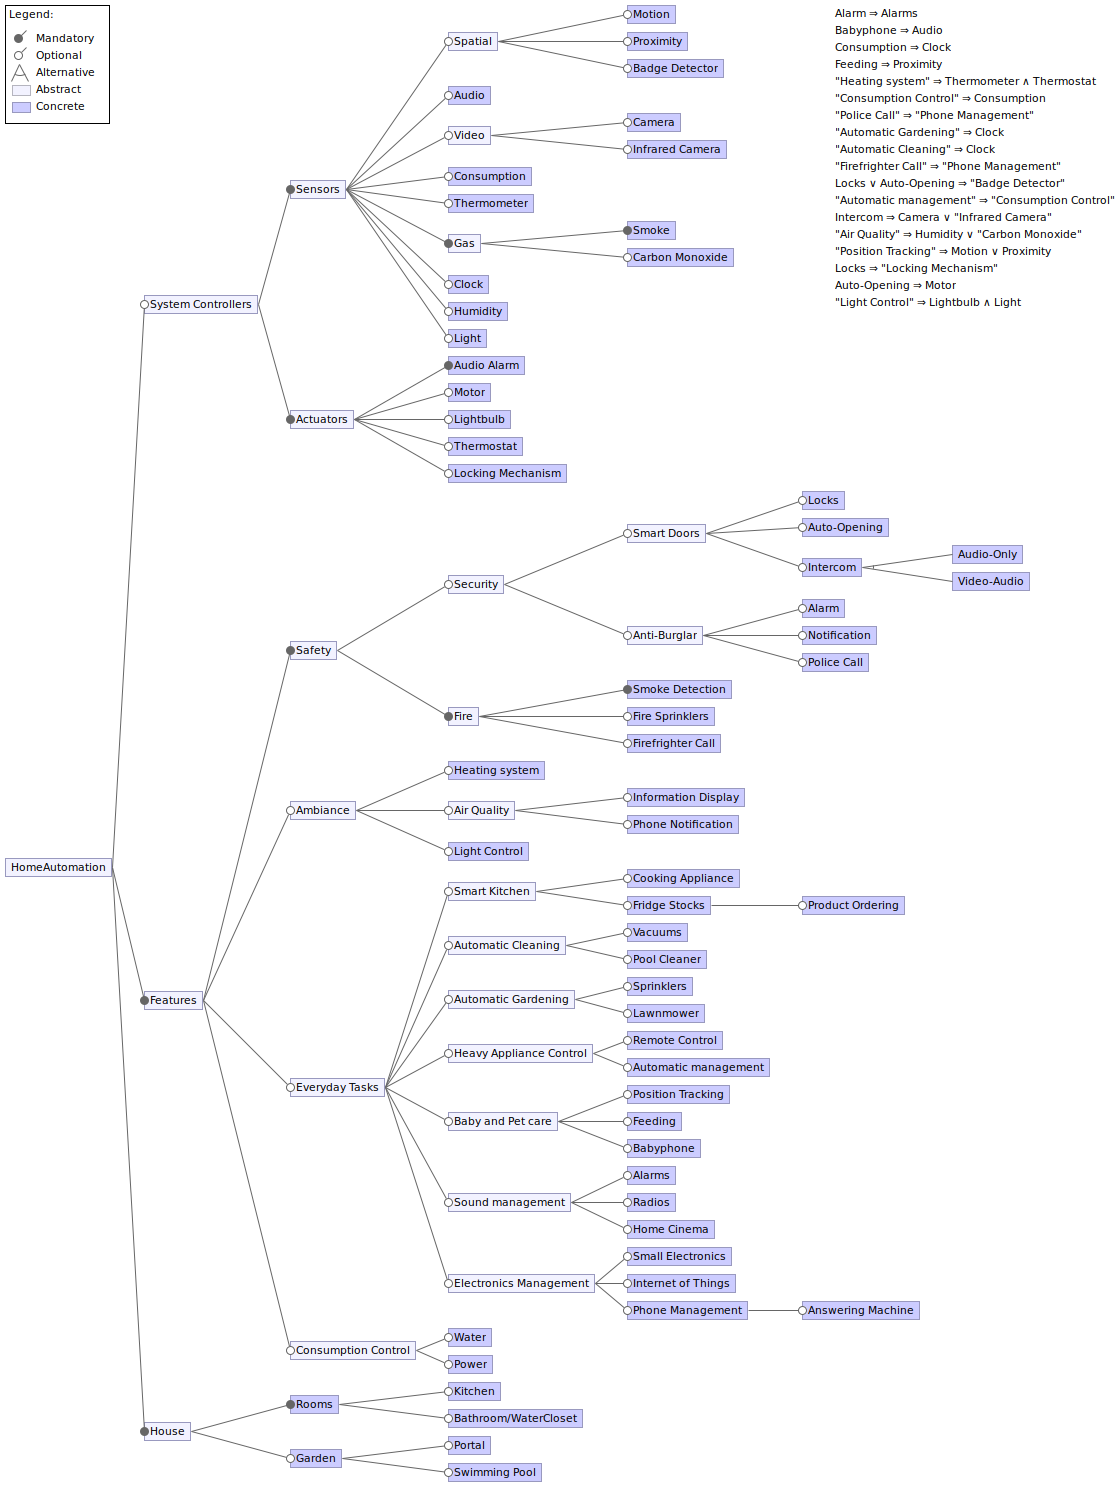
\includegraphics[width=0.9\textwidth]{FeatureModel_2.png}
        \end{figure}

\end{document}
